\section{Metrological reports}
 \label{s:metrological_reports}
Every page of the report shall use \SI{25}{mm} left, right, top and bottom page margins, unless this is impractical, and paragraph spacing should be single, except where otherwise stated. 
 
Paragraphs within the body text shall be separated by a single blank line and have no indentation.

Headings within the body text shall be followed by a 1.5-line width vertical space. The body text will follow immediately on the next line, without indentation.

\subsection{Printing and binding}
All paper report pages shall be printed single-sided.  The front page will use one of the standard MSL report front covers (see below), normal white paper will be used for the body of the report. A clear cover will be placed over the front page and an MSL report back cover will be added after the last page. The report will be bound using a white binder clip.

\subsection{Report covers}
 \label{ss:report_covers}
There are several MSL report front covers: use the one that gives the highest level of endorsement possible to ALL the reported results – any exception must be approved by the Chief Metrologist or Quality Manager.

\begin{itemize}
\item	A plain report cover for calibration, test or verification reports of measurements that are not covered by MSL's IANZ accreditation;
\item	An IANZ-endorsed \textit{calibration laboratory} cover for calibration reports of measurements that are included in MSL's IANZ accreditation, but not included in the CMCs in the BIPM database;
\item	An IANZ- and BIPM-endorsed \textit{calibration laboratory} cover for reports of measurements included in MSL's IANZ accreditation as well as the CMCs in the BIPM database;
\item	An IANZ-endorsed \textit{laboratory} cover for test or verification reports of measurements included in MSL's IANZ applied physics accreditation scope.
\end{itemize}

Note that when an endorsed report is being issued that contains some results outside the current scope of accreditation, the text under the IANZ logo must be:
\begin{quote}
\textit{All measurements reported herein, unless otherwise noted, have been performed in accordance with the laboratory's scope of accreditation.}
\end{quote}

\paragraph{Issuing body and traceability statement}
All covers include the following statements:

\begin{quote}\begin{minipage}{.7\textwidth}
ISSUED BY: \\
\textbf{Measurement Standards Laboratory of New Zealand} \\[\baselineskip]
Established under the Measurement Standards Act 1992 and\\
the National Standards Regulations 2019 to provide uniform\\ 
measurement of physical quantities throughout New Zealand.\\

All results quoted in this report are directly traceable to the\\
national measurement standards held by the Measurement\\ 
Standards Laboratory of New Zealand (MSL). MSL is New\\ 
Zealand's national metrology institute and operates within\\ 
Callaghan Innovation.
\end{minipage}\end{quote}

\subsection{Front page}
The front (cover) page:
\begin{itemize}
\item	must have ``Page 1 of [number of pages]'' printed in the top left-hand corner in bold;
\item	may have a job reference directly below the page number in bold;
\item	must have a title, which should be about one-third distance down the page and left aligned in bold;
\item	may have an identification for the instrument(s), e.g. serial number, either as part of the title or elsewhere on the front page;
\item	must have a report number that follows the title after two blank lines; 
The report number format is left-aligned and in bold font: register name/calendar year (yyyy)/sequential number (obtained from section report register), followed by report date; e.g. Temperature/2009/853, 21 January 2009.
\end{itemize}

\subsection{Header and footer on subsequent pages}
There will be a 2-line header, with: 
\begin{itemize}
\item	``Measurement Standards Laboratory of New Zealand'' centred and printed in bold on the first line; 
\item	in the second line, the report number and date are aligned to the left margin, and the page number [of pages] is aligned to the right margin;
\item	there should be 1.5-line width spacing between the lines.
\end{itemize}
The footer will contain the following warning about copying; the text will be centred, in italic, and use two lines (see also Appendix 1 in IANZ Procedures and conditions of accreditation \cite{IANZ_PC}): 
\begin{quote}
\centering\textit{This report may not be reproduced, except in full, without the written consent of the Chief Metrologist, Measurement Standards Laboratory of New Zealand.}
\end{quote}

\subsection{Second page}
The body of the second page begins with four blank lines followed by the report title, in bold, followed by another blank line.

\subsection{Signature page}
The last page of the main body of the report contains the signatures, as described below. Note, the signatures page does not have to be the last page of the report. Appendices, such as drawings, graphs or tables may be included following the signatures page.

The signatures page of the report shall be signed by the workers who contributed to the report, the checker who reviewed it and the Chief Metrologist (or delegate) who authorizes it. These individuals shall also initial all other pages of paper reports, but this not required for electronic reports.

For IANZ-endorsed reports, at least one of the workers or the checker signing the report must be a \deprecated{recognised IANZ signatory for the measurement class(es)} \proposed{Key Technical Person for the technical procedure(s)}  covering the measurements.

The person signing as Chief Metrologist, or for the Chief Metrologist, must be identified as such:  for the Chief Metrologist, use the label ``Chief Metrologist''; for a delegate use ``for Chief Metrologist''.

It is not necessary to identify the function of everyone signing the report.\footnote{This was a requirement under 17025:2005, but not in 17025:2017.}  However, a title (such as ``Technical Officer'', ``Scientist'', ``Electrical Metrologist'') and/or a subject area descriptor (e.g., photometry, temperature, etc.) may be used.

If a worker or checker is unable to sign the report, approval must be sought from that individual before signing \textit{per persona} (p.p.). A record of that approval must be kept with the job file.

\subsection{Report structure}
The report body may include the following headings, where relevant:
\begin{quote}
\begin{tabbing}
\textbf{Description}\hspace{12mm}\=including manufacturer (either a list or a proper sentence)\\[\baselineskip]

\textbf{Identification}\mbox{}\\[\baselineskip]

\textbf{Client}\mbox{}\\[\baselineskip]

\textbf{Date(s) of Test or Date(s) of Calibration}\mbox{}\\[\baselineskip]

\textbf{Objective}\mbox{}\\[\baselineskip]

\textbf{Method}\mbox{}\\[\baselineskip]

\textbf{Conditions}\mbox{}\\[\baselineskip]

\textbf{Results}\mbox{}\\[\baselineskip]

\textbf{Notes}\mbox{}\\[\baselineskip]

\textbf{Uncertainty}\mbox{}\\[\baselineskip]


\textbf{Conclusion}\>\begin{minipage}[t]{.7\textwidth}
(statements of fact only, such as verification of compliance with a documentary standard or regulation)\\[\baselineskip]
For example:\\

This gauge complies with the accuracy requirements of BS1780:1985\\ or an industrial gauge. (Paragraph 7.2.1 of BS1780: 1985 requires\\ hat the error in pressure indication shall not exceed \SI{1}{\%} of the\\ 
maximum scale value at any point above \SI{10}{\%} and below \SI{90}{\%} of the \\
maximum scale value, i.e. an error of \SI{36}{psi} in this case. The error\\ 
over the rest of the scale shall not exceed \SI{1.5}{\%} of the maximum scale\\ 
value, i.e. an error of \SI{54}{psi}.)\\

or\\

The measured mass values of these weights lie within the maximum\\ 
permissible limits for Class M1 as stated in IOML International \\
Recommendation No. 20. 

\end{minipage}
\end{tabbing}
\end{quote}

The report shall state the number of the technical procedure used, including the version number, for example: ``The weights were compared against reference standards of known mass and density following procedure MSLT.M.001.005.''  This reference may be contained, for instance, in a section entitled Technical Procedure, or in the Method section.

\subsection{Re-issued reports}
 \label{ss:reissued_reports}
Clause 7.8.8.1 of 17025:2017 requires that any change of information in re-issued reports be clearly identified and, where it is appropriate, the reason for the change should be given. We offer some guidance on how to do this here, however, other approaches may be acceptable.
\begin{enumerate}
\item	A new page can be inserted as page 2 of the report. This will contain a section titled ``Reissue Statement'' and identify the changes. The reason for inserting a whole new page is that it may avoid changes to the page layout of the original report (although pages numbers will be different).
\item	A decision about how to identify the changes needs to be made. When considering this question, assume that the client will not need to identify the difference between the old and new reports on more than one occasion. So, avoid over-highlighting changes. Nevertheless, it may be appropriate to tag or otherwise highlight individual changes embedded in other details. 
\end{enumerate}
The following is an example.

\textbf{\large Reissue Statement}\\

This report has been re-issued with the following changes:
\begin{enumerate}
\item	In the header of pages 2 to 8, the year incorrectly given as 2018 (but the year on title page 1 was correct).  The original date in the header is now written as ``27 May \sout{2018} 2019'' and the date of re-issue has been added.  
\item	The units reported in the first column of Table 1, Table 2 and the Table of Uncertainties of the original report were reported as mm. The correct units are inch. 
\item	Some values in Table 1 were incorrect. Values that have changed are indicated by a double dagger symbol $\ddagger$ (unicode 2021 – type 2021, then press alt-X), for example $0.93\,\ddagger$.
\item	There is a grammatical error in the final paragraph of page 4 (`include' has been changed to `includes').
\end{enumerate}  

\subsection{Fonts}
\subsubsection{Microsoft Word}
In Microsoft Word, the following fonts should be used.

On the front page, the Arial Narrow font is used, and all text is in bold. The sizes are as follows:
\begin{itemize}
\item	page number and job reference are set in 12-point, 
\item	the title is set in 18-point, and 
\item	the report number is set in 16-point.
\end{itemize}
The header and footer on all subsequent pages use 10-point Times New Roman font. The first line of the header is in bold; the warning in the footer about copying is in italic. 

The title on the second page uses Arial Narrow font and is set in 16-point bold.

In the main body of the report, the headings use Arial Narrow font and are set in 14-point bold. The body text uses 11-point Times New Roman font.
 
The Symbol font should be used as appropriate.

\subsubsection{Other text processors}
The Arial typeface has licensing terms that prohibit free redistribution, so the Arial font family is not always available on text processing systems. There are however, look-a-likes that provide satisfactory alternatives.

\subsection{Out-of-scope results (IANZ and CIPM MRA CMCs)}
It is acceptable to issue an IANZ-endorsed report that contains a small proportion of results outside the MSL accredited scope. In such cases, the text on the report cover under the IANZ logo must indicate that not all results are within scope (see \S\ref{ss:report_covers}) and the out-of-scope results must be clearly identified in the report (e.g., by adopting a distinctive notation or highlighting). If the out-of-scope nature relates to smaller uncertainties claimed, the report should also indicate a value of uncertainty that would be within scope.

It is acceptable to issue a report with the CIPM MRA logo containing a small proportion of results that are not covered by CMCs published in the Appendix C section of the BIPM key comparison database (KCDB). Those items shall be clearly identified as not being supported by the CIPM MRA (e.g., by adopting a distinctive notation or using a grey background on tables or figures).

\subsection{Informal reporting of measurements}
 \label{ss:informal_reporting}
On rare occasions, MSL may report measurements without fully applying the procedures of the quality system. 

Such reporting must be authorized by the Chief Metrologist.

One situation where informal reporting may be acceptable is in the context of scientific collaboration, which might ultimately result in publication of MSL measurements. Another possibility is during the manufacturing of a product, where early detection of deviations from design targets may be very helpful.

Informal reporting may lighten the overhead associated with issuing MSL calibration reports. Nevertheless, quality principles should still be applied (checking of technical procedure and data, traceability to the SI, etc).

The purpose of this policy is to protect clients, and MSL, from any undesirable outcomes arising from incorrect use of data that has been provided informally. Our quality system is intended to eliminate mistakes. Bypassing that system increases the risk that data contains errors. MSL trades on its reputation. The reputational risk to MSL, of a mistake being associated with our work, must be considered and discussed with the Chief Metrologist.

All data provided informally shall be accompanied by a disclaimer notice. This notice shall make clear that MSL does not stand by the quality of the data provided, which should not be used to inform critical decisions. 

A template for the disclaimer follows. This text may be adapted to different situations (words in bold font between square brackets can be modified appropriately, the other text in square brackets may be used, or modified, if appropriate). The final text must be approved by the Chief Metrologist.

\begin{quote}
\textit{The [\textbf{data reported on}] is provided `as is', without warranty of any kind, to [\textbf{recipient}] for [\textbf{purpose}] only. [{The data shall not be made publicly available, nor provided to a third party, without the consent of the MSL Chief Metrologist.}] [The data should not be used to inform any critical decisions.] This disclaimer must accompany any copies of the data.}
\end{quote}

\subsection{Electronic reports}
 \label{ss:electronic_reports}
 
An electronic report can be viewed on screen, or printed, by a client. We assume here that an electronic report is a PDF file representing a calibration report. 

The format of an electronic report must comply with the same general report formatting guidelines given in this document. 

The cover page will include one of the standard MSL report covers as a background image (watermark).

Electronic reports are produced by word-processing software (Word, LaTeX, etc), but electronic signatures are added to the PDF report in a distinct phase of the report issuing process, which uses different software. The two aspects-–-production and signing-–-must be handled separately. 
 
This section describes how to: 
\begin{itemize}
\item	add an MSL report cover to the background of a cover page in a Word document, and
\item	how to add electronic signatures to a PDF report, and 
\item	how to calculate a numerical code (MD5) for a particular file, which can be used to verify the integrity of file later.
\end{itemize}

\subsubsection{How to add an MSL report cover in Word}
\begin{enumerate}
\item	The cover page and the body of the report should be created as different Word ``sections''. 

(In the case of a new Word document that does not yet have section breaks, insert a `Next Page' section break on the first page -- using the `Breaks' drop-down list on the Layout tab.)
\item 	The MSL report cover image should be loaded as a custom Watermark from the design tab (figure~\ref{fig:word_watermark_dialog}). Select the \SI{100}{\%} scaling and uncheck the washout tick box. Then select and load the image file (accept to work off-line, if prompted).

\begin{figure}[h]
\centering
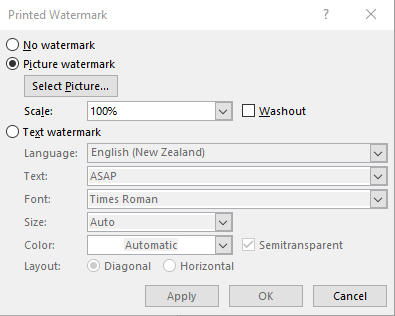
\includegraphics[scale=1]{pictures/word_watermark_dialog}
\caption{Word dialog box for adding a watermark.}
\label{fig:word_watermark_dialog}
\end{figure}
\item	The watermark will appear a bit washed out on the screen; don't worry, that's just to remind you it is in the background. 

However, the watermark will now appear on every page-–-read on. 
\item Open the header of the first body page (not the cover page) by double clicking in the header region. Then, deselect the ``Link to Previous'' button on the Header and Footer tab (If the ``Link to Previous'' button is disabled, don't worry, just proceed). 

Select the background image and delete it. The image on the cover page will remain. 

\end{enumerate}

\subsubsection{Signing an electronic report}
A signature image can be placed in a PDF file using \href{https://acrobat.adobe.com/nz/en/acrobat/pdf-reader.html}{Adobe Acrobat Reader DC}.
\begin{enumerate}
\item Open the PDF report file with the Reader. Select the ``Fill \& Sign'' option from the tools available (may be visible on the right, or else in the Tools menu)
\begin{center}
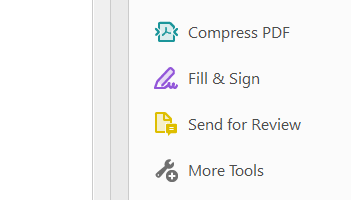
\includegraphics[scale=1]{pictures/acrobat_signing}
\end{center}
\item Select the ``Fill and sign'' option, when presented with the choice:
\begin{center}
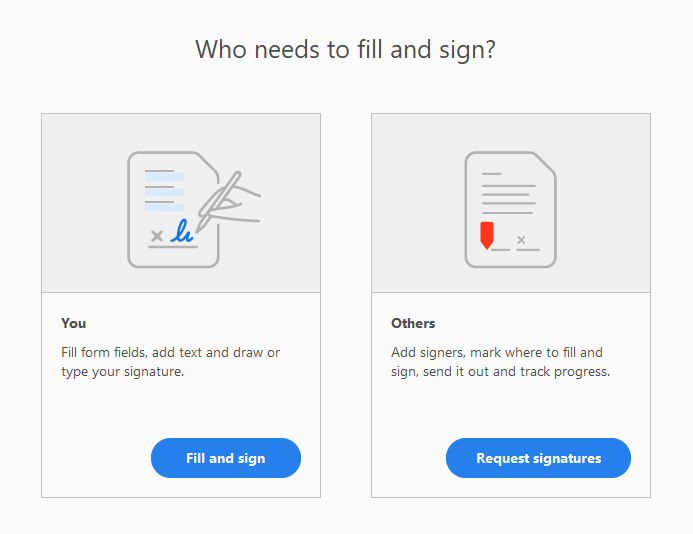
\includegraphics[scale=.6]{pictures/acrobat_signing_2}
\end{center}
\item A signing tool bar appears: 
\begin{center}

\includegraphics[scale=1]{pictures/acrobat_signing_3}
\end{center}
Go to the signature page of the report and click on the fountain pen icon, marked ``sign''. 

If it is the first time the Reader software is being used, you will need to load a signature file. Otherwise the software will present you with the image used last time. 
\item Click on the signature then place it in the document. A simple menu allows you to resize the image afterwards, if necessary. 
\begin{center}
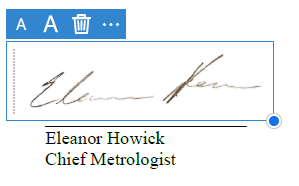
\includegraphics[scale=1]{pictures/acrobat_signing_4}
\end{center}
\item Save the file.
\end{enumerate}

\subsection{Checking the integrity of a report file}
 \label{ss:file_integrity_md5}
 
Under 17025, there is a responsibility to manage the integrity of documents. Errors can occur during transmission of electronic records. It is also possible to edit PDFs with some software.

One way to prove that a file has not been changed is to use an MD5 checksum \cite{MD5}. This is a code (a hexadecimal number) that can be calculated for any file. By keeping a record of the MD5 code of the signed report, we can check the integrity of a file later (e.g., after being emailed to a client). 

A checksum can be calculated in the Windows console, using the command ``CertUtil''. Here is an example:
\begin{center}
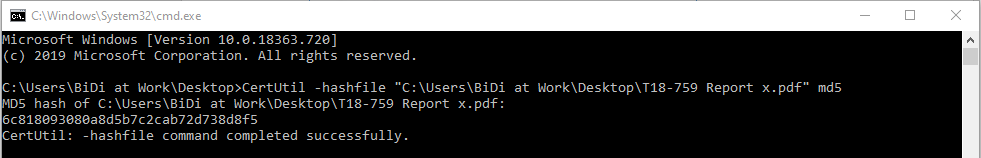
\includegraphics[scale=.6]{pictures/md5_cmd}
\end{center}
The command takes the form: 
\begin{quote}
\texttt{
> CertUtil -hashfile "\textit{Windows file path}" md5}
\end{quote}
The checksum result is the number \texttt{6c818093080a8d5b7c2cab72d738d8f5}.
 
There are many ways to calculate a checksum. Here is a simple Python script that takes a file path as input argument on the command line and prints the checksum (wil work in Python 2 or 3):

\begin{center}
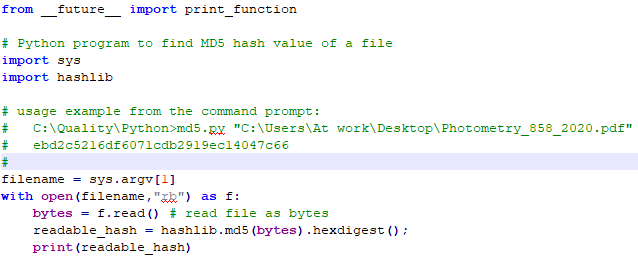
\includegraphics[scale=.8]{pictures/md5_python}
\end{center}

